\documentclass[../report.tex]{subfiles}
\begin{document}
    
    \begin{frame}
        \frametitle{6: Challenge Problem}
        \begin{figure}[!htb]
            \centering
            \frame{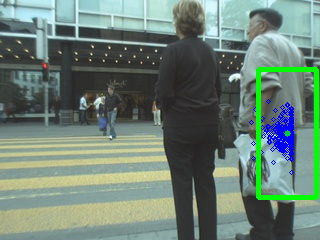
\includegraphics[keepaspectratio,height=0.65\textheight,width=0.45\textwidth]{ps5-6-a-1}}
            \caption{ps5-6-a-1}
        \end{figure}
    \end{frame}

    \begin{frame}
        \frametitle{6: Challenge Problem (cont.)}
        \begin{figure}[!htb]
            \centering
            \frame{
\includegraphics[keepaspectratio,height=0.65\textheight,width=0.45\textwidth]{ps5-6-a-2}}
            \caption{ps5-6-a-2}
        \end{figure}
    \end{frame}

    \begin{frame}
        \frametitle{6: Challenge Problem (cont.)}
        \begin{figure}[!htb]
            \centering
            \frame{
\includegraphics[keepaspectratio,height=0.65\textheight,width=0.45\textwidth]{ps5-6-a-3}}
            \caption{ps5-6-a-3}
        \end{figure}
    \end{frame}

    \begin{frame}[t]
        \frametitle{6: Challenge Problem Text response}
        \begin{normalsize}
            \begin{itemize}
                \setlength\itemsep{1em}\fontsize{6pt}{6pt}

                \item[]{\textbf{\selectfont\textcolor{blue}{ Describe what you did. Did this task present any additional challenges compared to the previous sections?  Include details about any modifications you had to apply. }}}
                
                \item[]\textbf{\documentclass[../report.tex]{subfiles}
\begin{document}
    
    \begin{frame}
        \frametitle{6: Challenge Problem}
        \begin{figure}[!htb]
            \centering
            \frame{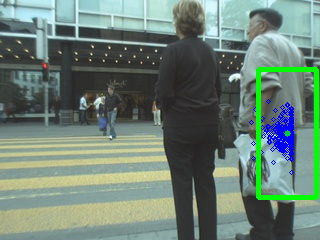
\includegraphics[keepaspectratio,height=0.65\textheight,width=0.45\textwidth]{ps5-6-a-1}}
            \caption{ps5-6-a-1}
        \end{figure}
    \end{frame}

    \begin{frame}
        \frametitle{6: Challenge Problem (cont.)}
        \begin{figure}[!htb]
            \centering
            \frame{
\includegraphics[keepaspectratio,height=0.65\textheight,width=0.45\textwidth]{ps5-6-a-2}}
            \caption{ps5-6-a-2}
        \end{figure}
    \end{frame}

    \begin{frame}
        \frametitle{6: Challenge Problem (cont.)}
        \begin{figure}[!htb]
            \centering
            \frame{
\includegraphics[keepaspectratio,height=0.65\textheight,width=0.45\textwidth]{ps5-6-a-3}}
            \caption{ps5-6-a-3}
        \end{figure}
    \end{frame}

    \begin{frame}[t]
        \frametitle{6: Challenge Problem Text response}
        \begin{normalsize}
            \begin{itemize}
                \setlength\itemsep{1em}\fontsize{6pt}{6pt}

                \item[]{\textbf{\selectfont\textcolor{blue}{ Describe what you did. Did this task present any additional challenges compared to the previous sections?  Include details about any modifications you had to apply. }}}
                
                \item[]\textbf{\documentclass[../report.tex]{subfiles}
\begin{document}
    
    \begin{frame}
        \frametitle{6: Challenge Problem}
        \begin{figure}[!htb]
            \centering
            \frame{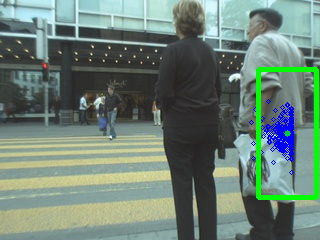
\includegraphics[keepaspectratio,height=0.65\textheight,width=0.45\textwidth]{ps5-6-a-1}}
            \caption{ps5-6-a-1}
        \end{figure}
    \end{frame}

    \begin{frame}
        \frametitle{6: Challenge Problem (cont.)}
        \begin{figure}[!htb]
            \centering
            \frame{
\includegraphics[keepaspectratio,height=0.65\textheight,width=0.45\textwidth]{ps5-6-a-2}}
            \caption{ps5-6-a-2}
        \end{figure}
    \end{frame}

    \begin{frame}
        \frametitle{6: Challenge Problem (cont.)}
        \begin{figure}[!htb]
            \centering
            \frame{
\includegraphics[keepaspectratio,height=0.65\textheight,width=0.45\textwidth]{ps5-6-a-3}}
            \caption{ps5-6-a-3}
        \end{figure}
    \end{frame}

    \begin{frame}[t]
        \frametitle{6: Challenge Problem Text response}
        \begin{normalsize}
            \begin{itemize}
                \setlength\itemsep{1em}\fontsize{6pt}{6pt}

                \item[]{\textbf{\selectfont\textcolor{blue}{ Describe what you did. Did this task present any additional challenges compared to the previous sections?  Include details about any modifications you had to apply. }}}
                
                \item[]\textbf{\documentclass[../report.tex]{subfiles}
\begin{document}
    
    \begin{frame}
        \frametitle{6: Challenge Problem}
        \begin{figure}[!htb]
            \centering
            \frame{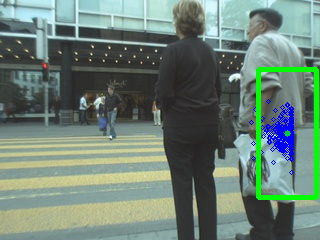
\includegraphics[keepaspectratio,height=0.65\textheight,width=0.45\textwidth]{ps5-6-a-1}}
            \caption{ps5-6-a-1}
        \end{figure}
    \end{frame}

    \begin{frame}
        \frametitle{6: Challenge Problem (cont.)}
        \begin{figure}[!htb]
            \centering
            \frame{
\includegraphics[keepaspectratio,height=0.65\textheight,width=0.45\textwidth]{ps5-6-a-2}}
            \caption{ps5-6-a-2}
        \end{figure}
    \end{frame}

    \begin{frame}
        \frametitle{6: Challenge Problem (cont.)}
        \begin{figure}[!htb]
            \centering
            \frame{
\includegraphics[keepaspectratio,height=0.65\textheight,width=0.45\textwidth]{ps5-6-a-3}}
            \caption{ps5-6-a-3}
        \end{figure}
    \end{frame}

    \begin{frame}[t]
        \frametitle{6: Challenge Problem Text response}
        \begin{normalsize}
            \begin{itemize}
                \setlength\itemsep{1em}\fontsize{6pt}{6pt}

                \item[]{\textbf{\selectfont\textcolor{blue}{ Describe what you did. Did this task present any additional challenges compared to the previous sections?  Include details about any modifications you had to apply. }}}
                
                \item[]\textbf{\input{yourAnswers/6.tex}}
            \end{itemize}
        \end{normalsize}
    \end{frame}

\end{document}}
            \end{itemize}
        \end{normalsize}
    \end{frame}

\end{document}}
            \end{itemize}
        \end{normalsize}
    \end{frame}

\end{document}}
            \end{itemize}
        \end{normalsize}
    \end{frame}

\end{document}